\documentclass[border=2pt]{standalone}
\usepackage{times}
\usepackage{amsmath,amssymb}
\usepackage{tikz}
\usetikzlibrary{arrows.meta,calc,positioning}
\begin{document}
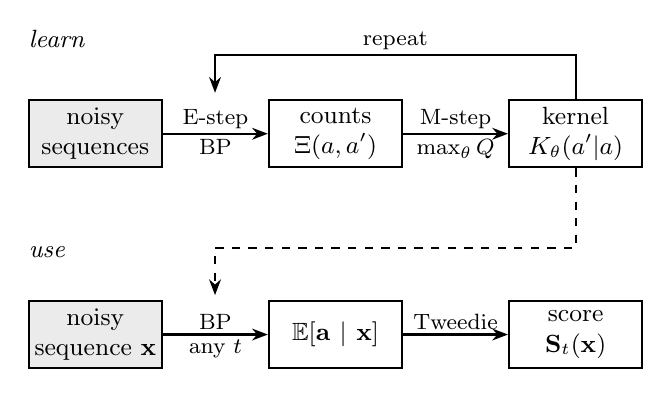
\begin{tikzpicture}[
    box/.style={draw,thick,align=center,font=\small,minimum height=8.5mm,inner sep=2pt,text width=1.55cm},
    data/.style={box,fill=black!8},
    arr/.style={-{Stealth[length=2mm]},thick},
    lab/.style={font=\footnotesize,align=center,inner sep=1.5pt},
    stage/.style={font=\small\itshape,anchor=west,inner sep=0pt}]
  \node[stage] at (-0.85,1.2) {learn};
  \node[data] (x) at (0,0) {noisy\\ sequences};
  \node[box] (xi) at (3.05,0) {counts\\ $\Xi(a,a')$};
  \node[box] (k) at (6.1,0) {kernel\\ $K_\theta(a'|a)$};
  \draw[arr] (x) -- node[lab,above]{E-step} node[lab,below]{BP} (xi);
  \draw[arr] (xi) -- node[lab,above]{M-step} node[lab,below]{$\max_\theta Q$} (k);
  \draw[arr] (k.north) |- node[lab,above,pos=0.75]{repeat} (1.52,1.0) -- (1.52,0.52);
  \node[stage] at (-0.85,-1.5) {use};
  \node[data] (y) at (0,-2.55) {noisy\\ sequence $\mathbf{x}$};
  \node[box] (m) at (3.05,-2.55) {$\mathbb{E}[\mathbf{a}\mid\mathbf{x}]$};
  \node[box] (s) at (6.1,-2.55) {score\\ $\mathbf{S}_t(\mathbf{x})$};
  \draw[arr] (y) -- node[lab,above]{BP} node[lab,below]{any $t$} (m);
  \draw[arr] (m) -- node[lab,above]{Tweedie} (s);
  \draw[thick,dashed,-{Stealth[length=2mm]}] (k.south) |- (1.52,-1.45) -- (1.52,-2.05);
\end{tikzpicture}
\end{document}
